\chapter{Background}

\begin{center}
    ``If you wish to make an apple pie from scratch, you must first invent the Universe.'' \\
    - Carl Sagan \cite{Video-SaganQuote}
\end{center}

\par Before one can begin to explore a problem, one must understand some of the underlying history and details related to the problem. Additionally, it is beneficial to explore aspects of the solution as well. In this chapter, a history of multiple parts of this project - the technical aspects (\gls{cg}, \gls{xr}, \gls{hci}, Software Engineering) and the application aspects (\gls{hud}, \gls{hdd}, Automobiles) - are explored.

\section{XR, CG, and HCI}
    \par Ivan Sutherland, an early pioneer in the fields of \gls{cg} and \gls{vr}, once said, ``The screen is a window through which one sees a virtual world. The challenge is to make that world look real, act real, sound real, feel real.'' \cite{Book-Garassini1994} In this context, the ``screen'' Sutherland is referring to is the literal screen of a computer - the display. In Sutherland's early days (1960s), a computer display would have been a \gls{crt}. When paired with a keyboard, it would become an interface into a remote time-shared computer.

    \par Before Sutherland's landmark doctoral dissertation - ``Sketchpad, A Man-Machine Graphical Communication System''. \cite{Thesis-Sketchpad}, the field of computer graphics was considered still in its infancy. In his thesis, Sutherland introduced new, interesting concepts related to the way people interacted with machines. The graphics used in Sketchpad were very primitive - basic, un-shaded 2D polygons. The interface for the Sketchpad system was also revolutionary, yet very primitive by today's standards. A light pen - a device that uses sensors to detect light on a screen, along with a series of manually controlled limit switches, and a monitor, were used to create, display, and manipulate Sketchpad's graphics. Yet, even with all of the primitive aspects of the system, many of today's commonplace software development techniques and attributes were introduced, either explicitly or implicitly - interactive computer graphics, object-oriented programming, and non-procedural programming languages. \cite{Video-KayExplainsSketchpad} Even through all of the progress that was made, it would be some time before CG would become anything that would be considered close to realism.

    \begin{figure}[h]
        \vspace{0.5cm}
        \centering
        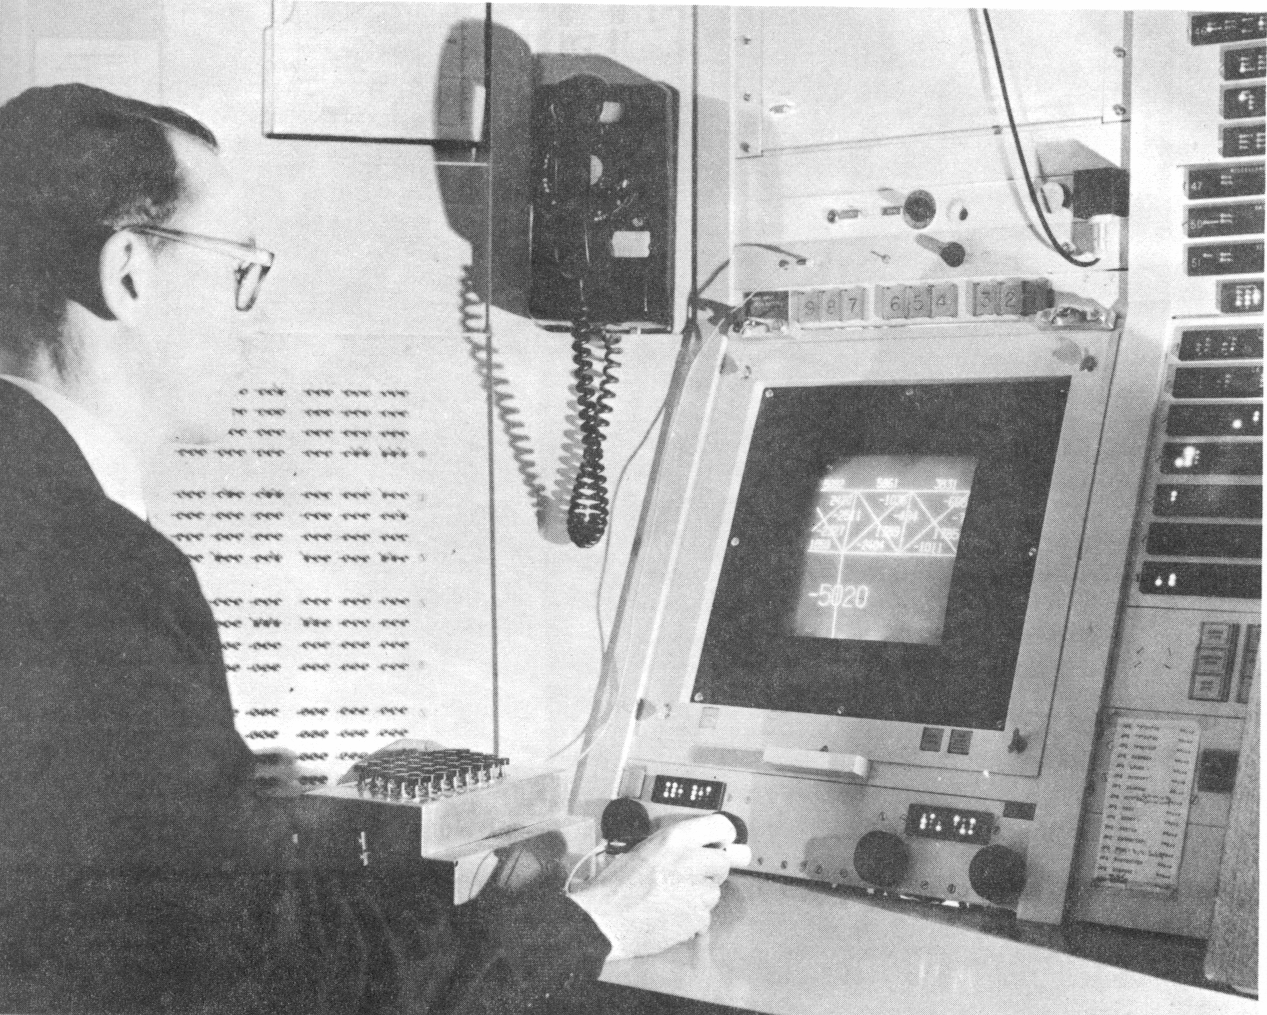
\includegraphics[scale=0.75]{./Support/Images/SketchpadDissertation.png}
        \caption{Demonstration of Sketchpad (1963). \cite{Image-SketchpadDemo}}
        \label{figure-sketchpaddemo}
    \end{figure}

    \par A little over a decade after Sketchpad, a Ph.D candidate at the University of Utah explored new and efficient means of producing curved surfaces. The student, Edwin Catmull, advised by Sutherland himself, produced what is considered another landmark piece - A Subdivision Algorithm for Computer Display of Curved Surfaces. \cite{Thesis-Subdivision} He, along with other University of Utah students, later co-founded an animation company known as Pixar Animation Studios, known for their award-winning animated films and advancements in computer animation technology (e.g. RenderMan \cite{Web-Renderman}). Many now standard computer graphics technologies and techniques either came from or were enhanced by Pixar - ray tracing (the projection of light in virtual environments) \cite{CP-DistributedRayTracing}, model texturing enhancements \cite{TP-TextureOnDemand}, and others.

    \par Other efforts, while not \gls{cg}-centric, utilized \gls{cg} in innovative and expressive ways. In the early 1970s, Terry Winograd - Computer Science Professor Emeritus at Stanford University and renowned expert in \gls{hci} - developed a \gls{cg}-based \gls{ai} program called SHRDLU. \cite{Web-SHRDLU} While innovative, SHRDLU was limited to a micro-world containing basic elements - blocks, pyramids, and a box. Each element was given a color. These colors could be used as an identifier of a group of elements (e.g. all red objects), or in conjunction with a specific element (e.g. the red pyramid). The earliest implementation lacked any shading of the graphics, which made it difficult to track elements. However, later efforts by students at the University of Utah introduced color rendering of the micro-world's graphics, thus improving the comprehension of the environment. \cite{Web-SHRDLU} In retrospect, this micro-world could be considered a primitive representation of the physical world around us; rather, a form of world simulation.

    \par In all of these efforts which shaped the fields of \gls{xr}, \gls{cg}, \gls{hci}, and implicitly, the field of computing in general, one must recognize the organized, collaborative efforts of the software engineers and artists behind the screen. Without software engineering, these feats would not have been possible.

\section{Software Engineering and the Agile Model}
    \par While \gls{xr} and \gls{cg} have had revolutionary and evolutionary changes over the course of time, software engineering has followed a similar pattern. The term ``software engineering'' was coined by Margaret Hamilton - one of NASA's programmers during the Apollo missions to the moon. \cite{Web-HamiltonSoftwareEngineeringTerm} While her contemporaries were against the phrase, perceiving software engineering as a ``fad'', the field has emerged in a rapid and very expansive fashion. What solidified this new field of engineering, and prevented it from falling into obscurity, was its structured approach to design, implementation, and testing. Other engineering disciplines are known for such practices.

    \par One of the greatest tools at the disposal of a software engineer is a development model - a structure process flow in which software is developed. One of the earliest software engineering models was the Waterfall development model. Waterfall is comprised of sequential, interdependent processes. \cite{Book-SoftwareEngineeringSommerville}

    \par Waterfall begin with requirements gathering. \cite{Book-SoftwareEngineeringSommerville} In this phase, the software engineer determines the problem and needs of the users. In private development, a software engineer would interview the end users for the details of what the software system should and should not do. For larger, public-oriented developments, market research and feedback on a larger scale is necessary. During this time, a feasibility study may be performed. This will allow a software engineer to determine if the proposed work is even technically feasible, given the state of computing technology at that point in time. Generally, and ideally, a software engineer may work within the confines of a defined software stack - a set of software which offers the resources necessary to make a user-level application. Consistent software stacks promote software that's easier to maintain and consistent across an organization. \cite{Book-SoftwareEngineeringSommerville}

    \par Once these requirements are gathered, the next phase of the Waterfall is the System Design. \cite{Book-SoftwareEngineeringSommerville} During this phase, many technical details are explored and defined. What technology required to develop a solution to the problem? Are data sources needed? How is the data stored and retrieved? How will the user interacts with the software? Many other questions and possibilities are analyzed and explored. During this phase, a series of documents may be produced which explain processes and procedures for system function and interaction. These documents, generally referred to as \gls{uml} diagrams \cite{Web-UMLIntro}, define, in a clean, consistent fashion, system behavior, user expectations, and technical solutions. Once a majority of the pending questions are answered, and design documents are complete, a software design is realized. The implementation phase begins. \cite{Book-SoftwareEngineeringSommerville}

    \par Implementation is the process of developing a software solution based on the generated design. \cite{Book-SoftwareEngineeringSommerville} If the software design is of high quality (i.e. concise details, defined use cases, etc.), a software engineer should be able to implement a solution relatively fast. If the design is low quality (i.e. lacking detail, holes in information, technically infeasible, etc.), a lot of unnecessary time can be spent implementing a solution that does not meet the requirements initially established. It is important for quality to be preserved throughout the entire process, so the most effective solution can be implemented as efficiently as possible. \cite{Book-SoftwareEngineeringSommerville} During implementation, the software engineer adheres to their organization's practices and standards when programming, as well as those defined by their stack's respective standards (i.e. \glsxtrshort{posix} if using a UNIX-based operating system, \glsxtrshort{tcpip} if developing a web application, etc.). Again, such guidelines and rules help promote the development of clean, consistent applications.

    \par Once the implementation is complete, the software is thoroughly tested. \cite{Book-SoftwareEngineeringSommerville} This process requires the software engineer to try the use cases defined in the Design phase, and verify they can be successfully achieved. Erroneous conditions are also tested (invalid inputs, out of order operations, etc.). This is to verify the software can handle and/or recover from the potential faults, or gracefully terminate. As software issues (colloquially known in the software engineering community as ``bugs'') are found, the software engineer proceeds to adjust the solution accordingly. Eventually, after refinement is complete, a hopefully stable product is created, and ready for release and longer term maintenance - the final phase of Waterfall. \cite{Book-SoftwareEngineeringSommerville}

    \par Once released, the end users begin using the solution. As time progresses, more bugs may be discovered, or new features may be requested. Depending on the structure of the software and context of the solution, the same software engineer who designed and implemented the solution may also perform the maintenance operations. In larger organizations and for public software, another software engineer may perform the maintenance, depending on the availability of the original source code. Some organizations rely on multiple people to achieve the same end result. Product/Program Managers, Software Analysts, and other design-oriented roles may perform the Requirements Gathering and System Design. Software Developers/Engineers may solely implement a solution. Quality Assurance (QA) engineers and testers verify the software's integrity and function. Each role, feeding into the next, achieved by a collective group.

    \par While Waterfall provided an effective, familiar means of implementing a software solution, it is not perfect. One of its issues is its general flow - sequential, very detail driven from the start, thus generally resulting in longer development times. While this process works for some solutions, other solutions require a faster means of software release and maintenance. A variant of Waterfall, named ``Modified Waterfall'', offers a means of backtracking to either gather more requirements, refine the design, or re-implement part or all of the solution. While this may help with some of the initial needs (i.e. missed requirements, oversights in design, etc.), it may extend a software solution's release even further, or may prevent a release at all.

    \par Some individuals saw the Waterfall model, and decided they could implement a better version of it. That model would become Agile Software Engineering. \cite{Book-SoftwareEngineeringSommerville} Agile attempts to resolve some of the issues of Waterfall. While it follows the same phases as Waterfall, the phases are handled a lot faster, in smaller chunks, and with respect to time constraints. Agile models are broken into cycles, or ``sprints''. During a sprint, software engineers attempt to fully implement a defined solution. These solutions, again, are a lot smaller than those in Waterfall. Based on the results of the cycle, more cycles may be needed to extend, enhance, re-implement, or remove functionality. However, in turn, the software is released in a more rapid fashion, users can provide feedback faster, and maintenance is continuously ongoing to improve the solution.

    \par Practical examples of Agile being used in society can be found in the heart of Silicon Valley. Companies such as Google \cite{Book-SoftwareEngineeringAtGoogle} and Facebook \cite{TP-FacebookDevelopmentAndDeployment} utilize a ``quick and often release'' mentality, enabled through the use of Agile development. While this sounds potentially reckless and unprofessional, this model of development has the potential to uncover and correct issues faster than traditional Waterfall-based models.

    \par Now that the basis of what \gls{xr}, \gls{cg}, and Software Engineering are have been established, let's proceed to explore a use case involving all of these elements. A composition of these technologies can result in a solution that satisfies a very practical, essential problem faced in society today - reducing distractions while driving an automobile.
